\documentclass[12pt]{memoir}
\usepackage{common}

\addbibresource{references}

\title{}
\author{Andrew Head}

\begin{document}

\begin{center}
Understanding and Advancing How Programmers Learn from,\\ Design With, and Reuse Online Programming Examples
\end{center}
\vspace{-1ex}

\definition{Author}{Andrew Head, PhD Student, UC Berkeley}

\definition{Keywords}{code examples; code reuse; learning from examples;}

%%% Introduction

An amazing body of comprehensive, high-quality online documentation has grown in the last decade~\cite{parnin_crowd_2012,mamykina_design_2011} that has made it easier than ever for programmers to consult the web to find examples of unfamiliar languages and APIs~\cite{brandt_two_2009}.
And while such resources seem like a boon in all regards, observation of programmers reusing examples has revealed a practice fraught with hazards.
When programmers learn the bare minimum to do a coding task, they write shoddy code to just satisfy the intended functionality, reimplement code stable libraries could support, and spend more time debugging copied code~\cite{brandt_opportunistic_2008,brandt_two_2009}.

The code example has been identified by many CS education researchers as a cornerstone of CS education (e.g.,~\cite{lahtinen_study_2005}).
Yet today, we do not understand the role that pervasive online code examples play in either the formative open-ended project-based work of CS upper division curriculum or industry work of freshly minted software engineers.
One reason is that reliance on online code examples has only recently been possible, in part due to the rapid growth of the massive, popular programing Q\&A StackOverflow, launched in 2008.

\if 0
Engaging with learning materials on the job is critical to a budding programmer's development as a professional~\cite{exter_exploring_2012}.
Current evidence of end-user challenges in reusing code examples outside of the classroom~\cite{brandt_two_2009} has provided anecdotal evidence of reuse pitfalls, but no systematic understanding of the impact of online code example reuse habits on learning, design, and code quality.
\fi

To gain a thorough understanding of how online code example use habits impact a programmer's learning, design ability, and code quality, I want to answer the following questions for the academic community:
When copying and pasting is easy, how often do programmers actually learn new concepts from code examples ($Q1$)?
How often can they design new code from the components used ($Q2$)?
How frequently do they reuse code that contains violations of idioms or undesirable side-effects ($Q3$)?
% How long does pasted code remain in use ($Q4$)?
What interventions can we envision to enhance programmers' ability to build mental models of the code they find ($Q4$), and support more successful reuse and modification of found code ($Q5$)?

%%% Problem statement

My proposed research seeks to \textbf{understand the affordances and pitfalls of programmers working with online code examples during informal learning, and to vigorously explore in-browser and IDE-based interfaces to support programmers in effectively learning from and using online examples.}

%%% The Approach

I will pursue $Q1$--$Q3$ applying standard observational and experimental techniques from HCI\@.
Following a method I have practiced in past work~\cite{head_tutorons_2015}, I will conduct controlled lab studies that ask programmers perform code reuse and modification tasks, with participants sampled from UC Berkeley EECS upperclass students.

$Q1$ and $Q2$ must be answered in a necessarily careful way---participants must be encouraged to program in a `typical' way that makes use of arbitrary online examples.
This means that programmers must be provided with a non-trivial, open-ended programming problem (e.g., building a chat server as in~\cite{brandt_two_2009}), as working with singular examples that the experimenters picked would result in atypical attention to examples.
A second assistant will be used to remotely watch the programming activity and formulate questions about randomly sampled APIs during the study session.
These can be asked at the end of the session to assess programmers' knowledge of and ability to build new solutions with APIs used.

$Q3$ requires access to copied-and-pasted code from realistic scenarios.
The experiments described above will be a first source of this.
Further information will be obtained by conducting contextual inquiries with project teams from UC Berkeley's upper division user interface design and implementation course, and collecting copy-and-paste information via a method similar to the apparatus described in~\cite{kim_ethnographic_2004}.

On top of this novel knowledge, I will explore the design space of web and IDE-based interfaces to better support learning, design, and high-quality integration of code found in online examples ($Q4$--$Q5$).
The interfaces will match the work habits I observed during the previous stages of study.

However, I expect these interfaces will take two major forms:
First, \emph{automatic, concise, and in-situ to significantly reduce the cost of finding the information needed to build a solid mental model of what code does}.
Infrastructure I built in past work~\cite{head_tutorons_2015} already provides a solid technical grounding and design patterns for generating English prose and usage examples to aid in explaining arbitrary online code snippets for a collection of small languages.
Second, \emph{interactions to foster close inspection of code prior to pasting} for programmers who lack training in systematic code inspection.
This may consist of developing novel in-browser note-taking methods (e.g.,~\cite{bauer_selection-based_2007}) and automatic question-asking (e.g.,~\cite{mitkov_computer-aided_2003}) methods.

This project will therefore yield insights into the learning, design, and programming challenges of programmers working with online code examples, and concrete software systems and techniques for explaining and encouraging engagement with this code.
This knowledge and these tools are critical to preparing the next generation of programmers to thrive in industry, for whom learning new skills ``on the job'' is a core competency~\cite{exter_exploring_2012}.
In this way, my work promotes the NSF broader impacts of \textbf{increasing and improving public engagement with science and technology}, and \textbf{improving STEM education}.

This research will contribute to the academic body of knowledge on end-user software engineering challenges and strategies, and programming tools to support modern paradigms of development.
Beyond related work that inspires the current work (e.g.,~\cite{brandt_two_2009,ichinco_exploring_2015}),
this research will address our community's need to understand the implications of code reuse of online examples on programmers' ability to develop mental models, design, and develop quality code.
I will disseminate our new knowledge of the affordances and pitfalls of online examples among the academic communities of CHI, VL/HCC, and CSE\@, and publish insights on the design and usability of the software artifacts at UIST\@.

%%% Intellectual Merit

% It is clear from my experience debugging code with students as a student instructor that reuse occurs frequently in the upper division CS classroom, and that hastily pasted code is the cause of confusion and errors.
% From speaking with other professors, this is no uncommon occurrence.
% While a large body of work in CS Education has proposed and evaluated curricula (e.g.,~\cite{tew_developing_2010}), assignments, and textbook examples (e.g.,~\cite{borstler_quality_2011}), the online code example is an important learning resource that we don't understand.

% The work we produce here will be disseminated by three major means.
% Finally, all programming tools developed will be made open source and available for immediate public use.

%%% Broader impacts


\if 0

\section{Background}

Clarke introduced the persona of an \emph{opportunistic developer} to describe the software developer who develops just enough of an understanding of a technology to solve a business problem~\cite{clarke_what_2007}.
Recent studies have observed opportunistic behavior for programmers beyond business, including creative workers~\cite{brandt_opportunistic_2008} and web designers~\cite{dorn_learning_2010}.
While this style of development enables rapid results~\cite{brandt_opportunistic_2008}, it comes with hazards:
functionality is copied and pasted from online examples, with less attention to explanations~\cite{brandt_two_2009};
code may be written in a sub-optimal way in order to maintain flow and move on to other tasks~\cite{brandt_opportunistic_2008}.
% programmers are more likely to re-implement functionality instead of reusing established systems and libraries~\cite{brandt_opportunistic_2008};

Past observation confirms that the cards are stacked against typical programming documentation for maintaining the attention of those developing opportunistically.
In human-computer interaction, Carroll writes how users learning new technologies are often too busy learning to make use of instruction~\cite{carroll_nurnberg_1990}.
For end user programmers (those programming for personal purposes~\cite{ko_state_2011}), Blackwell's Attention Investment models how programmers carefully weigh the costs of engineering activities against perceived benefits~\cite{blackwell_psychological_2006}.
Good software engineering practice, like understanding the model of an API, often loses to expediency.

When a programmer's focus centers on trial and error with code instead of making sense of comprehensive references, we face two tasks to better support the opportunistic developer in understanding found code.
First, \textbf{relevant documentation should be moved from hidden locations to the code examples they arre used in.}
Second, \textbf{documentation should be provided in a context-relevant, easy-to-read, short form.}

Meanwhile, a growing corpus of online high-quality ``crowd documentation''~\cite{parnin_crowd_2012} provides new environments in which to support context-relevant documentation and new resources to mine and serve to information seekers in a context-relevant form.

\section{Proposed Research}

I hypothesize that new techniques for delivering context-relevant, summative documentation will help opportunistic developers in two ways:
\begin{itemize}[noitemsep,topsep=0pt]
\item By decreasing verbosity and increasing relevance, it will enable programmers to gain the same understanding of libraries with less effort
\item When presented next to code examples, it can lesson the effort required to develop solutions involving unfamiliar software
\end{itemize}

I propose three systems to demonstrate the potential of context-relevant, summative programming documentation.
The \textbf{intellectual merit} of the first of these systems has already been recognized:
the Tutorons work has received an Honorable Mention VL/HCC~\cite{head_tutorons_2015}, a main conference on end user programming.
Prototypes for the other systems two have been built.
They must undergo substantial further development and evaluation.

\subsection{Tutorons}
% Context-relevant descriptions of online code found during opportunistic information seeking.
Programmers often encounter syntax that they don't understand in web tutorials that has not been explained by the tutorial author.
A Tutoron is a routine on a public server that can detect code snippets in the markup for tutorial pages, and synthesize English prose, diagrams, and usage examples to describe this code.
When a programmer navigates in a browser instrumented with the Tutorons plugin, programmers can view context-relevant explanations of high-level intent of code and its low level syntax for snippets automatically detected by the server.
Tutorons were implemented for three languages commonly embedded in tutorials: the wget Unix command line, CSS selectors, and regular expressions.
An initial in-lab usability study has shown that such adaptive explanations can reduce accesses to external documentation on the Web (Fisher's exact test, $n$ = 9, $p<.01$).
\andrew{As future work, this section can suggest recommending libraries, options and code that \emph{aren't} within the detected snippet.}

\subsection{StackSkim}
Often, there are many tutorials that can satisfy a programmer's information need, but the first one programmers find is not sufficient.
StackSkim is a visual search interface for exploring, comparing, and selecting code from large collections of similar examples, providing a front-end to millions of questions from StackOverflow, a popular programming Q\&A.
The system has yet to be applied to be comprehensively evaluated, and we seek to address two challenges:
(1) building algorithms and visual affordances to detect and highlight differences between snippets serving the same purpose
(2) interleaving examples with production code mined from Github to reveal common exception cases that occur in practice.
% It enables programmers to detect the most popular classes and programming structures used in collections of dozens of related answers to their questions, and locate examples with either minimal or elaborate accompanying explanation.
% A preliminary usability study revealed positive qualitative feedback, 
% The primary technical contribution for both of these steps will revolve around comparison of pre-parsed code examples from the relatively clean repositories of example and production code on StackOverflow and Github, respectively.

\subsection{CodeConverter}
When developing opportunistically, programmers rely on known languages to get work done~\cite{brandt_opportunistic_2008}.
\andrew{Check this reference---I'm not sure it's true.}
To reduce the barrier of working with unfamiliar languages within the same domain, we propose an experimental system called CodeConverter.
When learning a new language, programmers will write simple statements of a familiar language, and expand them to see the semantic equivalent in the target language.
With CodeConverter, a new language's syntax will be described through the translations that appear---relevant descriptions will be provided as comments accompanying expansions instead of as a tutorial with a preset path.
For feasibility, first studies will focus only on rule-based translation of small statements for restricted problem sets, rather than using machine translation (e.g.,~\cite{karaivanov_phrase-based_2014}).
% The eventual evaluation will focus on having programmers from a local hackerspace develop code for an embedded platform with an unfamiliar language but with familiar tasks.

Evaluation of each of these systems will include mixed methods.
Success of the tools in reducing programming effort will be measured by, for instance, task completion rates and reference to external documentation for in-lab usability studies with programmers.
Qualitative feedback will be collected from all studies to refine our understanding of programmer information seeking challenges and our systems' affordances.
The result will be a set of software artifacts to new programmer workflows for making use of documentation during opportunistic development.

\fi

\if 0
\begin{figure}%
  \centering
  \parbox{.45\textwidth}{%
    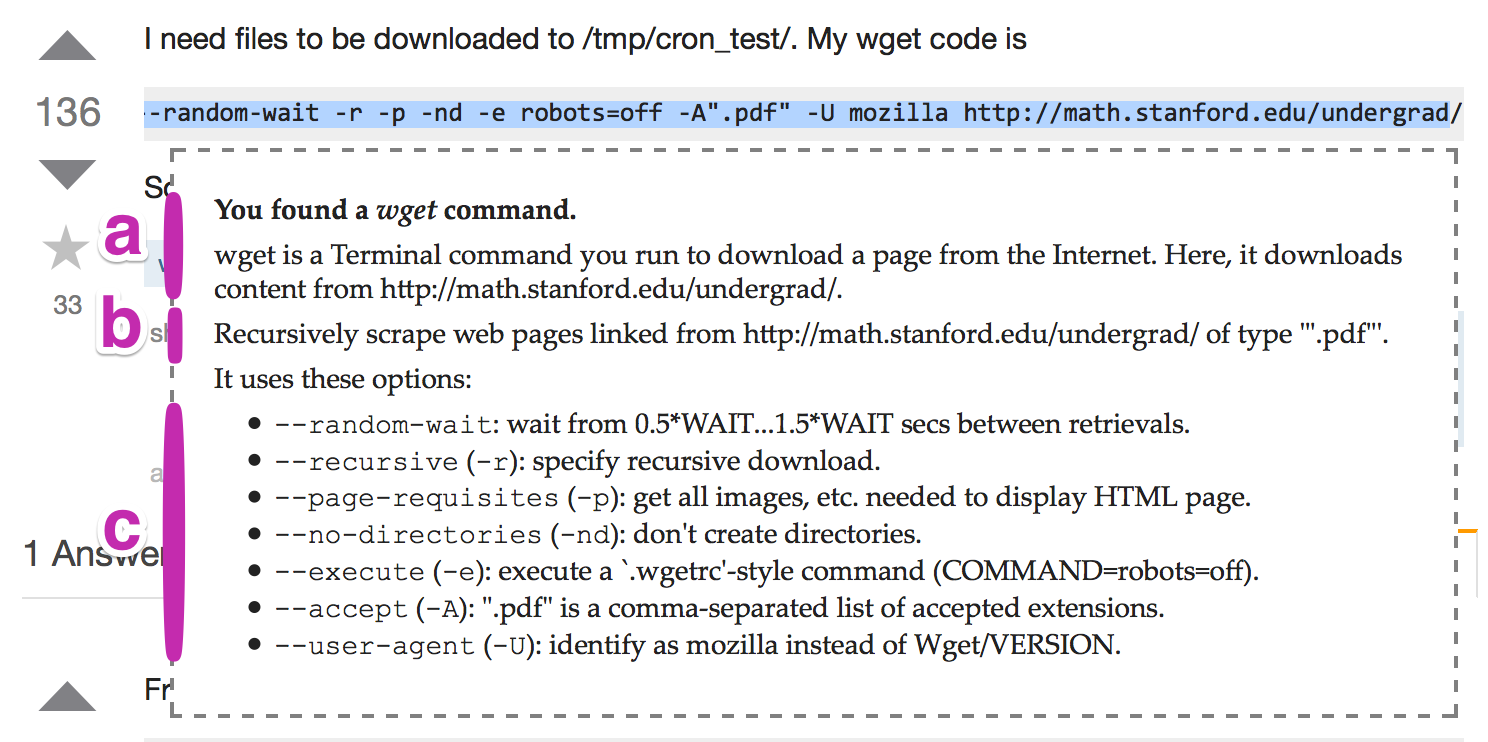
\includegraphics[width=\linewidth]{figures/tutorons_microexplanation}
    \caption{%
      A micro-explanation for a command line generated by a Tutoron with multiple levels of detail 
      (definition, high-level intent, arguments)
    }\label{fig:tutorons_microexplanation}
  }%
  \qquad
  \parbox{.45\textwidth}{%
    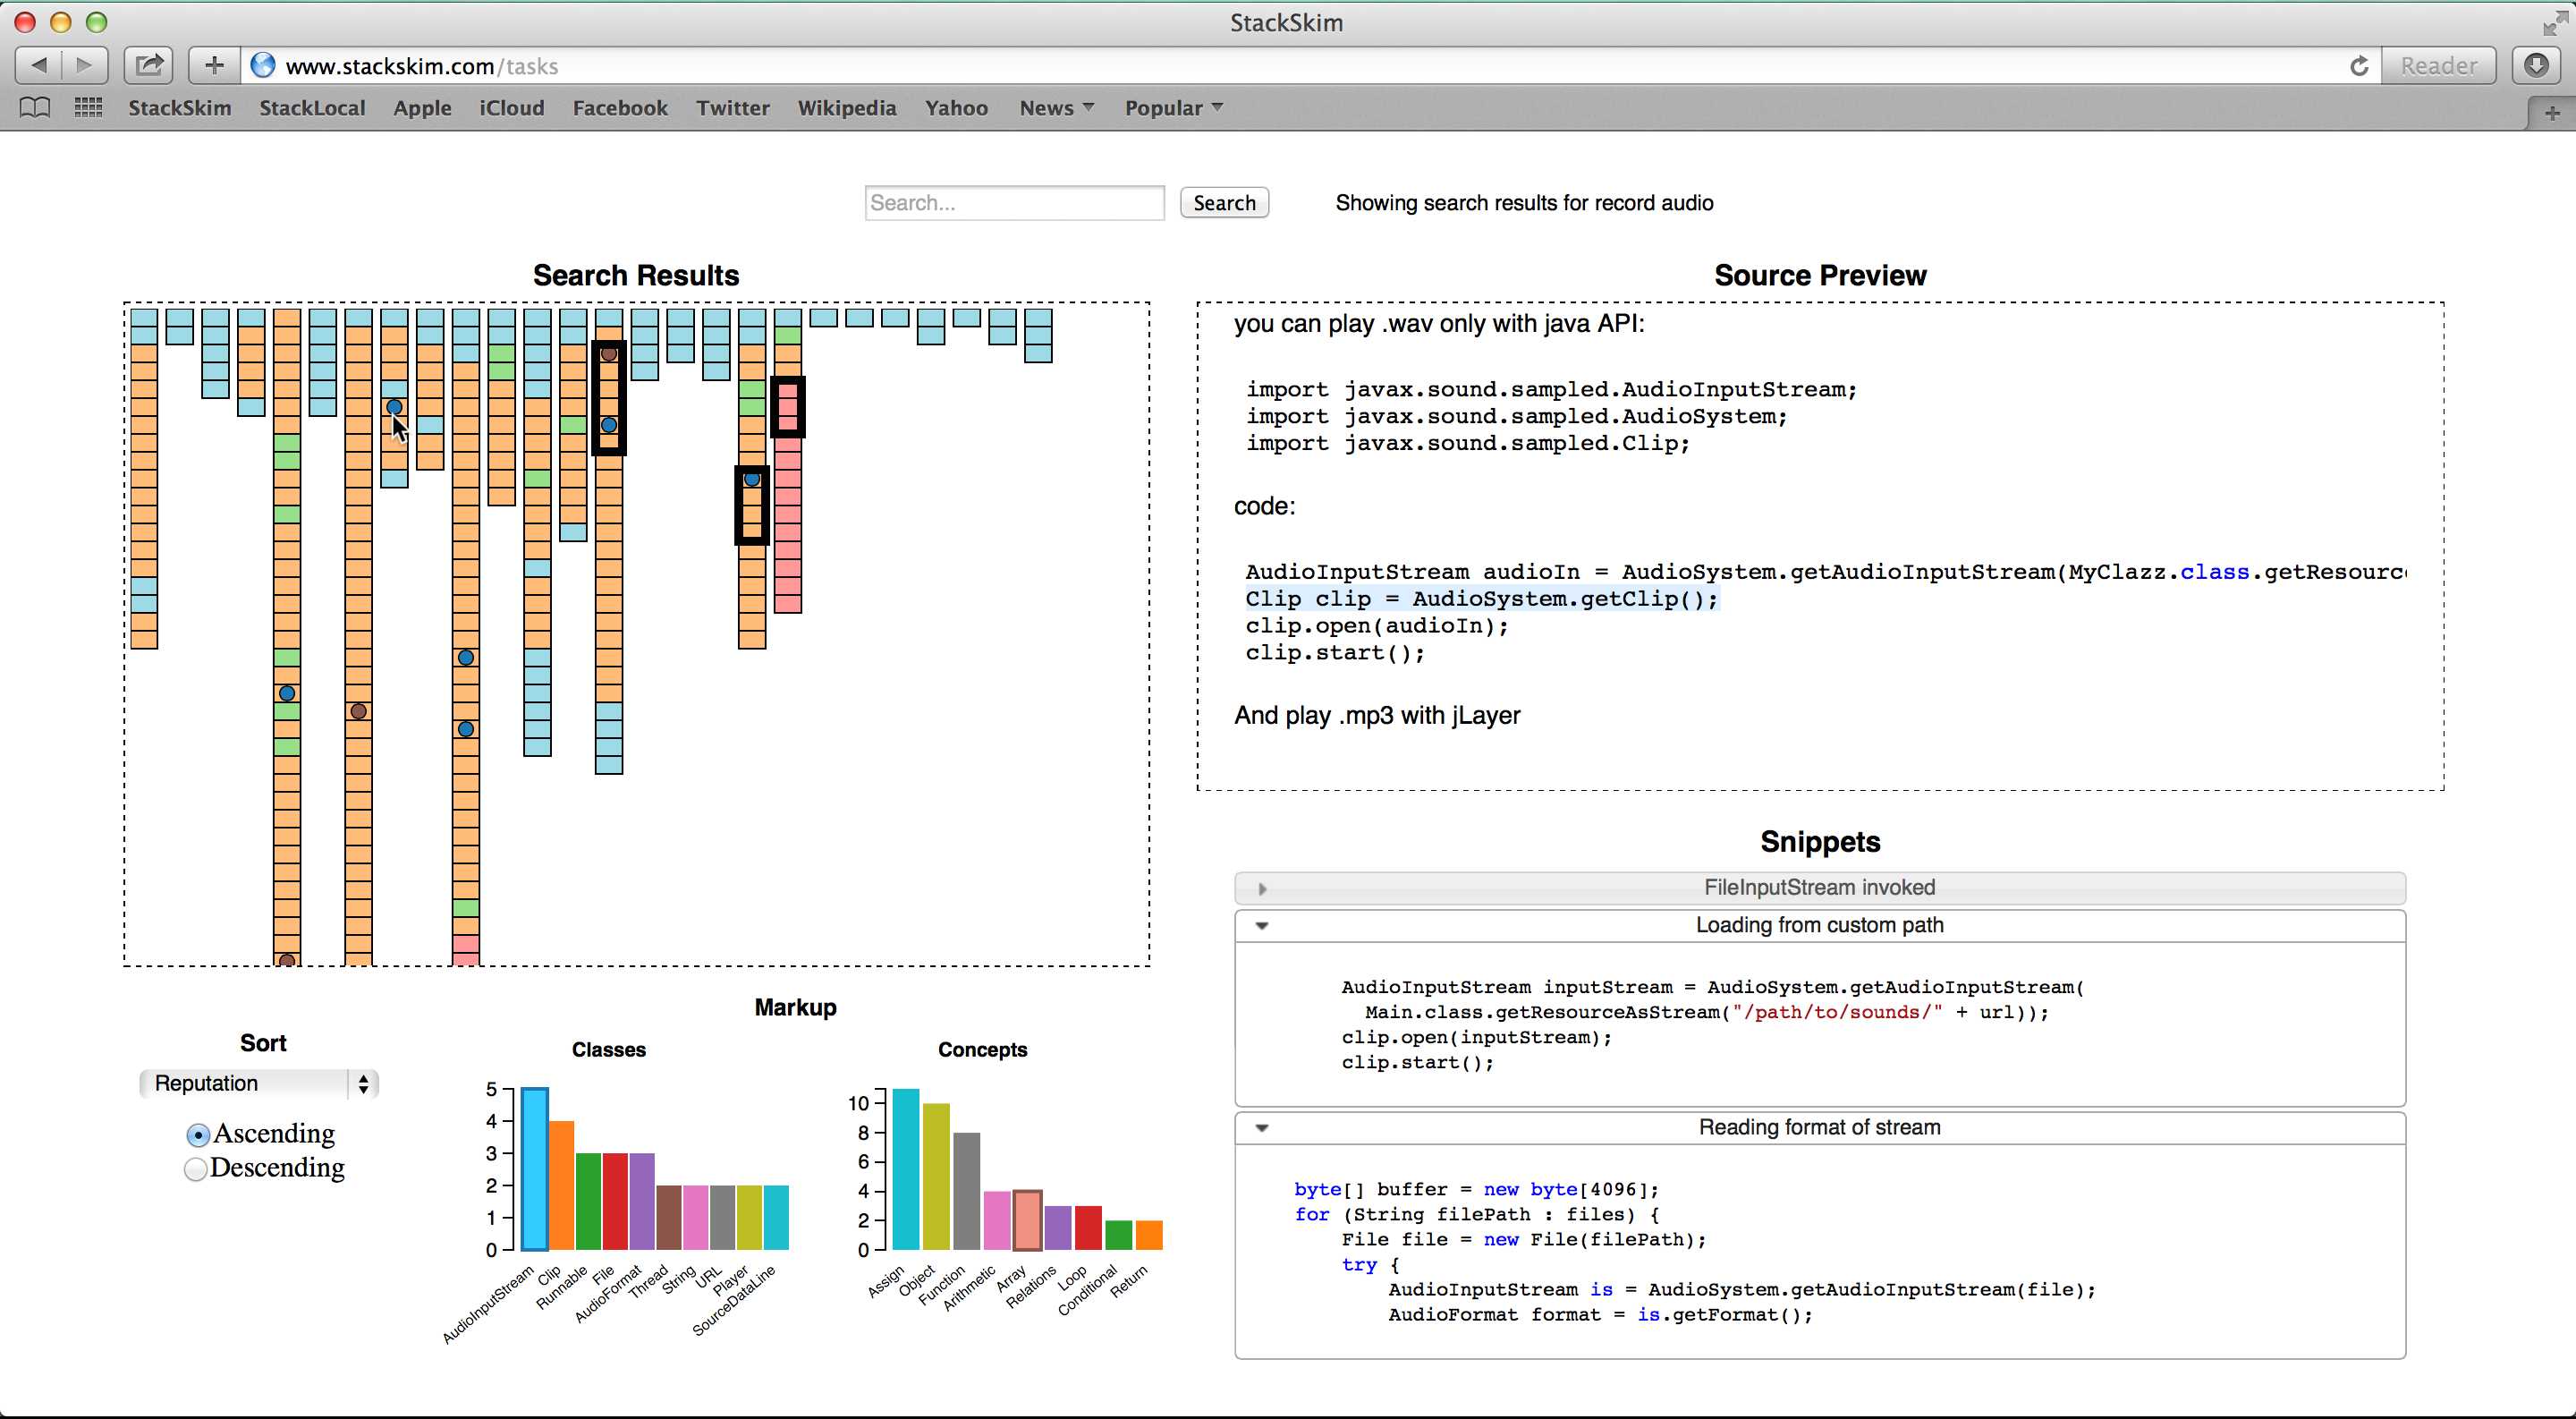
\includegraphics[width=\linewidth]{figures/stackskim_ui}
    \caption{%
      StackSkim, a visual interface for comparing and noticing trends in large collections of code examples that solve the same problem.
    }\label{fig:stackskim_ui}
  }
\end{figure}
\fi

\if 0
Point out the number of non-professional programmers.
Also point out crises in developing technologies that are caused by programmers who followed non-systematic practices

This work can be seen as an effort to reconcile the best practices of the ``systematic developer'' with recent tendencies of ``opportunistic'' programming habits.
\textbf{I could add in a mention of Blackwell's Attention Investment model here to mention why it is that programmers may program opportunistically, and why we should and how we can vary incentives and costs.}
Clarke introduced the persona of an \emph{opportunistic developer} to describe a software developer who writes code in an ``exploratory fashion'' and develops a ``sufficient understanding of a technology to understand how it can solve a business problem''.
(This contrasts with the \emph{systematic developer}, who writes code defensively and ``develops a deep understanding of a technology before using it''~\cite{clarke_what_2007}.)
In their study of exhibit designers at San Francisco's Exploratorium interactive science museum, Brandt et al.\ reported on a group who engaged in \emph{opportunistic programming} who weren't professional developers~\cite{brandt_opportunistic_2008} but were very much what might be considered as end-user programmers --- those developing code for personal rather than public use~\cite{ko_state_2011}.

Brandt et al.\ associated several habits with opportunistic programming that are counter to what we would hope for students working with code or end-users developing a better understanding of code.
Those programming opportunistically likely to incorporate functionality by copying and pasting code, often from online sources~\cite{brandt_two_2009}.
They are more likely to implement functionality from scratch for well-known libraries, instead of reusing existing systems and libraries~\cite{brandt_opportunistic_2008}.
They also practice ``code satisficing'', implementing functionality in a sub-optimal way in order to maintain flow and move on to other functionality~\cite{brandt_opportunistic_2008}.

While opportunistic programming is powerful in that it allows one to rapidly prototype and ideate and that it reduces the cycle time of editing and debugging code~\cite{brandt_opportunistic_2008}, this behavior discourages the formation of new mental models and an introduction to new tools that should be encouraged for both novice programmers and many end-user programmers.
The author of this proposal observed much of what would be called ``opportunistic'' habits while instructing a user interface design course.
After providing reference code to students for programming interfaces on Android phones and smartwatches, he helped students debug problems related to API reuse and the side effects of mixed code from multiple examples after hearing students self-report to having ``copied and pasted'' code from online tutorials and the slides he distributed.
In light of a prevalence of the ease of opportunistic habits and programmers' ability to copy-and-paste code from an increasingly comprehensive body of crowd documentation online~\cite{parnin_crowd_2012}, I define the goals of my research:

\emph{In my research, I develop and study software artifacts to support systematic inspection of found code from information interfaces programmers use when developing opportunistically.}

The theoretical deliverables of this work is establishing how systematic habits amidst opportunistic practice will improve:
(\emph{a}) programmers' mental models of reused code, libraries and tools used they develop
(\emph{b}) enable more accurate feasibility assessments of upcoming tasks (for example, see~\cite{ko_role_2011})
(\emph{c}) reduce design barriers~\cite{ko_six_2004} when planning new functionality

The artifacts that I develop belong to two themes:
\begin{itemize}[noitemsep]
\item Techniques for automatically generating instructive explanations and demonstrations of found code
\item Interfaces for critical inspection of alternatives when selecting code for reuse
\end{itemize}

I have developed the artifacts that enable exploration within both of these themes, and have published a first paper on the one of the two themes.
Toward the first, a paper I presented at VL/HCC explored techniques for automatically augmenting code in online examples with natural languages explanations and demonstrations of code.\footnote{%
The Tutorons system was implemented as both a browser plugin and a standalone JavaScript library, and can be viewed in action on \url{www.tutorons.com}.
}
We put forward a set of four guidelines to inspire the development of context-sensitive help:
(\emph{a}) leverage multiple representations to illuminate high-level intent and enable low-level understanding of syntax
(\emph{b}) be concise --- skip static explanations and focus on dynamically generated content
(\emph{c}) reappropriate existing documentation
(\emph{d}) inspect code examples on a large scale to support explanations of common usage.
In a nine-participant user study, the system was shown to reduce the number of accesses to external documentation needed to modify online code to perform new tasks.
\textbf{Next steps will include \ldots}
\textbf{Mention the theories used: MLT, layered documentation, Attention Investment}

Towards the second goal, I and co-developer have built a visual search interface for StackOverflow, a popular online programming Q\&A.
In response to Brandt et al.'s recommendations to develop tools that support ``comparing, reasoning about, integrating, and modifying found code''~\cite{brandt_opportunistic_2008}, we developed StackSkim, \emph{a visual search interface for exploring answers to StackOverflow questions that have a multitude of answers}.
The interface offers rapid visual inspection of frequent libraries used for addressing the searcher's programming problem;
through direct manipulation, users can also rapidly collect and compare similar code snippets.
\textbf{Next steps will include \ldots}

Each of these efforts relies on the cultivation of new software artifacts to aid programmers in understanding code during an opportunistic programming task.
Each has already followed and will continue to follow a mixed methods approach of observation and controlled experiments to determine how these tools indeed alter not only the task of opportunistic programming, but also programmers' behavior in selecting, understanding, and using code found online.
We are currently developing a version of Tutorons explanations that we hope will be incorporated into an introductory CS classroom's online textbook to better understand the role of automatic explanations of code for novice programmers.
\textbf{Add some note here about how we intend to run some workshop on clean code reuse habits.}
\fi

\section{References}
\printbibliography[heading=none]

\end{document}
